\subsection*{詳細設計}

次に、クラスごとの機能の設計を、クラス図を作成して行った。以下に詳細設計を示した、商品識別システムのクラス図\cite{v_model}を図\ref{class}に載せる。また、クラスごとの動作要件を満たす検証項目についても述べる。
\begin{figure}[htbp]
\centering
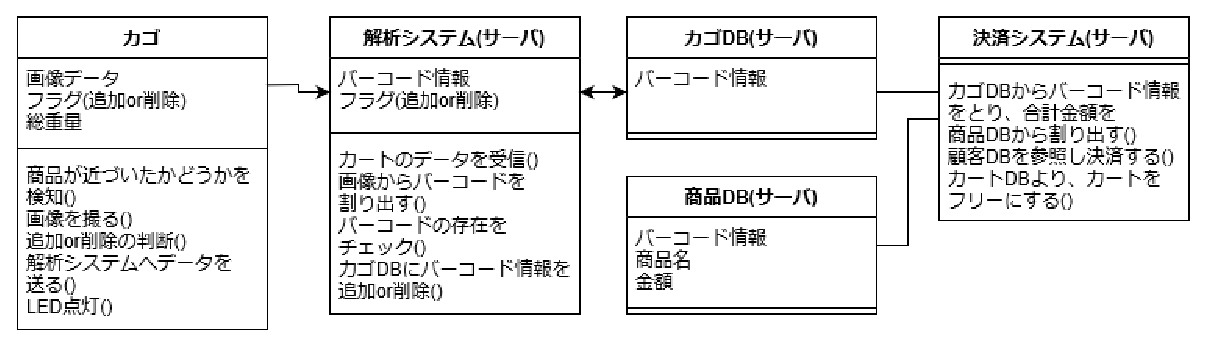
\includegraphics[width=15cm]{./pic/class_final.eps}
\caption{クラス図}
\label{class}
\end{figure}

図\ref{class}はカゴ、解析システム、カゴDB、商品DB、決算システム、それぞれの操作を示したクラス図である。カゴクラスでは、ユーザが商品を出し入れする際に、その商品の画像データを確保する。また、ユーザに解析が成功したかの通知を行う。解析システムクラスでは、カゴから送られてきたデータの受信、解析とカゴDBへの操作を行う。カゴDBでは、ユーザが購入予定の商品の管理を行う。商品DBでは、商品のバーコード番号と商品名、値などの商品情報を管理している。店側が新しい商品を追加する場合は、このDBに商品情報を追加する必要がある。最後の決済システムでは、ユーザが決済する際に必要な処理を行う。
 \ref{class}に記述されているクラスの具体的な機能と検証項目(単体テスト項目)について説明していく。
\begin{itemize}
\item カゴ
 画像データの取得方法を説明する。画像の取得は、カゴに取り付けられた距離センサとWebカメラを連動させて行う。
距離センサを使用すると、カゴに商品が接近したことを検知できる。センサが商品を検知後、Webカメラが画像を固定枚数撮
影する。次にフラグ(追加・削除)の取得方法を説明する。フラグの取得には重量センサを用いる。重量センサを使用するとセンサ上にある物体の総重量の検知が可能である。総重量が増加した場合は追加すると判断し、減少した場合は削除すると判断する。画像データとフラグ(追加・削除)の2つのデータの取得が完了すると、解析システムへデータを送る。
LEDの点灯は解析結果をユーザに通知するためものである。
\item カゴDB
 カゴDBは、購入予定商品のバーコード番号を管理する。このDBは解析システムによって操作される。また、決済システムによって決済が終了した場合は、データを削除する。
\item 商品DB
 この商品DBは、店側が新商品の追加や、値段の更新を行いたい場合に操作される。
\item 解析システム
 カゴクラスが解析に必要な、画像データとフラグ(追加・削除)を送信すると、解析システムがデータを受信して解析が始まる。画像データからバーコード番号の解析に成功すると、一緒に受信したフラグを使用して、カゴDBにバーコード番号を追加する。ただし、存在しない番号の追加を防ぐために、DBに追加する前に商品DBを参照し、該当するバーコード番号が存在する場合のみ追加を行う。また解析に成功した場合も、失敗した場合もカゴへ結果を送信する。
\item 決済システム
 決済システムは、ユーザが決済を行うときに動作する。ユーザが商品を出し入れする時点で、購入予定商品の情報がカゴDBに格納されているため、決済時にカゴの中にある商品を1つずつスキャンする必要はない。
\end{itemize}


次に、シーケンス図を用いてシステムの手順を説明する。以下の図\ref{sequence}にそって説明する。赤枠で囲っている部分が筆者の実装担当である。
図\ref{sequence}はカート側、サーバ側、Webページ側の3つに大別される。左から右の順に処理を行う。シーケンス図から読み取れるように、ユーザからカートへ商品が渡され、カートで処理を行う。処理が終わると解析システムへ情報が伝達され、解析が始まる。解析結果をカゴDBとカートに送信する。結果はWebページへ反映される。カートではDBの操作は行われない。

\begin{figure}[htbp]
\centering
\includegraphics[width=15cm]{./pic/sequence_final.eps}
\caption{シーケンス図}
\label{sequence}
\end{figure}